\vspace{-15pt}
% Comick v3.0 (TheFinalComick)
Plusieurs variantes du réseau pré-entraîné \emph{Resnet18}
\begin{center}

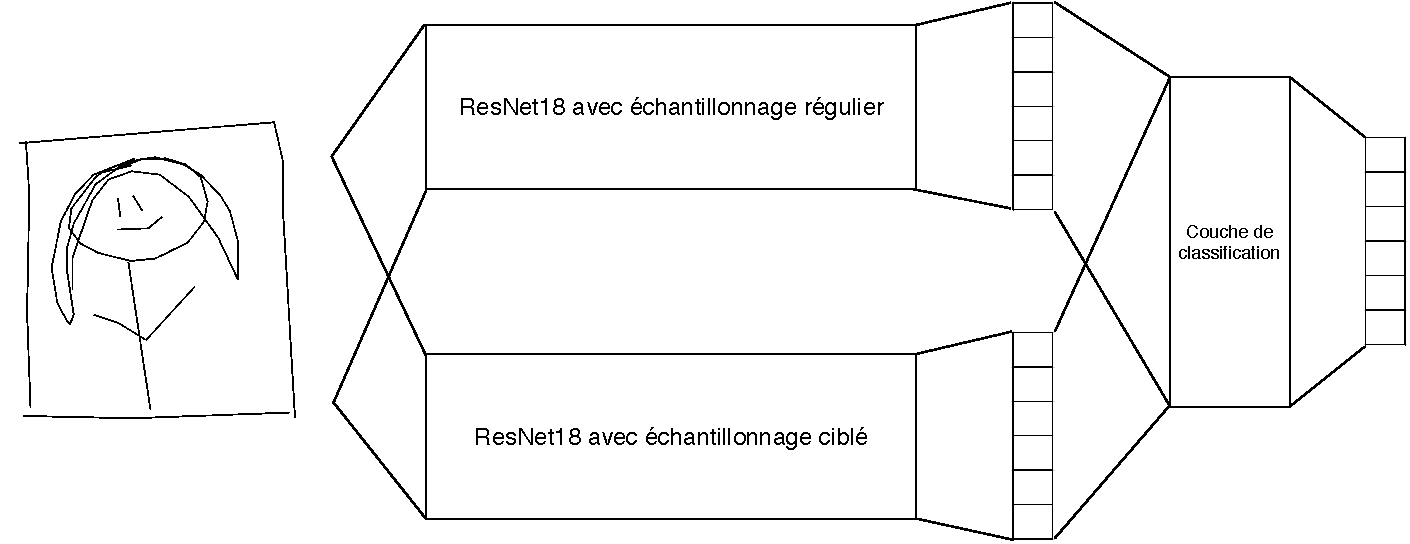
\includegraphics[width=30cm,height=30cm,keepaspectratio]{figures/structure_reseau.pdf}
      
\end{center}

Étant donné les contraintes, utilisations d'epochs non traditionnelles, chaque epoch consiste en un \textbf{échantillonnage d'un nombre fixe d'images par classe} (ex: 500 images aléatoires par classe: epoch de 170 000 données plutôt que le jeu complet).

Similaire à du \textbf{Bootstrapping} .


Variantes:

\begin{itemize}
\item Échantillonnage variant selon l'exactitude par classe: $N^*=N(1-accuracy) +0.25N$
\item Méthode par ensemble avec couche de classification
\item Méthode par ensemble avec moyenne
\end{itemize}